% Multiple Choice Question 4

\begin{center}
    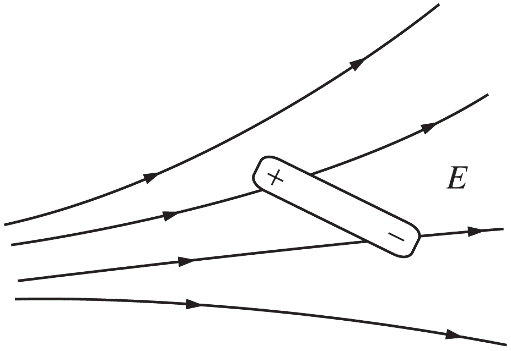
\includegraphics[scale=0.3]{images/img-003-002.png}
\end{center}

\begin{questions}
\setcounter{question}{3}

\question
An electric dipole consisting of a positive charge and a negative charge held a fixed distance apart is at rest in an external, nonuniform electric field $E$, as shown in the figure above. Which of the following best describes the net torque and net force exerted on the dipole?

\tabto{0.75cm} \underline{Net Torque}
\tabto{5cm}    \underline{Net Force}

\begin{choices}
    \choice Clockwise        \tabto{4.25cm} To the left
    \choice Clockwise        \tabto{4.25cm} To the right
    \choice Counterclockwise \tabto{4.25cm} To the left
    \choice Counterclockwise \tabto{4.25cm} To the right
    \choice Zero             \tabto{4.25cm} Zero
\end{choices}

\end{questions}
